%Version 3 October 2023
% See section 11 of the User Manual for version history
%
%%%%%%%%%%%%%%%%%%%%%%%%%%%%%%%%%%%%%%%%%%%%%%%%%%%%%%%%%%%%%%%%%%%%%%
%%                                                                 %%
%% Please do not use \input{...} to include other tex files.       %%
%% Submit your LaTeX manuscript as one .tex document.              %%
%%                                                                 %%
%% All additional figures and files should be attached             %%
%% separately and not embedded in the \TeX\ document itself.       %%
%%                                                                 %%
%%%%%%%%%%%%%%%%%%%%%%%%%%%%%%%%%%%%%%%%%%%%%%%%%%%%%%%%%%%%%%%%%%%%%

%%\documentclass[referee,sn-basic]{sn-jnl}% referee option is meant for double line spacing

%%=======================================================%%
%% to print line numbers in the margin use lineno option %%
%%=======================================================%%

%%\documentclass[lineno,sn-basic]{sn-jnl}% Basic Springer Nature Reference Style/Chemistry Reference Style

%%======================================================%%
%% to compile with pdflatex/xelatex use pdflatex option %%
%%======================================================%%

%%\documentclass[pdflatex,sn-basic]{sn-jnl}% Basic Springer Nature Reference Style/Chemistry Reference Style


%%Note: the following reference styles support Namedate and Numbered referencing. By default the style follows the most common style. To switch between the options you can add or remove �Numbered� in the optional parenthesis. 
%%The option is available for: sn-basic.bst, sn-vancouver.bst, sn-chicago.bst%  
 
%%\documentclass[sn-nature]{sn-jnl}% Style for submissions to Nature Portfolio journals
%%\documentclass[sn-basic]{sn-jnl}% Basic Springer Nature Reference Style/Chemistry Reference Style
\documentclass[sn-mathphys-num]{sn-jnl}% Math and Physical Sciences Numbered Reference Style 
%%\documentclass[sn-mathphys-ay]{sn-jnl}% Math and Physical Sciences Author Year Reference Style
%%\documentclass[sn-aps]{sn-jnl}% American Physical Society (APS) Reference Style
%%\documentclass[sn-vancouver,Numbered]{sn-jnl}% Vancouver Reference Style
%%\documentclass[sn-apa]{sn-jnl}% APA Reference Style 
%%\documentclass[sn-chicago]{sn-jnl}% Chicago-based Humanities Reference Style

%%%% Standard Packages
%%<additional latex packages if required can be included here>

\usepackage{graphicx}%
\usepackage{amsmath,amssymb,amsfonts}%
\usepackage{amsthm}%
\usepackage{mathrsfs}%
\usepackage[title]{appendix}%
\usepackage{xcolor}%
\usepackage{textcomp}%
\usepackage{manyfoot}%
\usepackage{booktabs}%
\usepackage{algorithm}%
\usepackage{algorithmicx}%
\usepackage{algpseudocode}%
\usepackage{listings}%
\usepackage{mathtools}
\usepackage{commath}
\usepackage{multirow}
\usepackage{caption}
\usepackage{bm}
\usepackage{siunitx}
\usepackage{makecell}
\usepackage{hhline}
\usepackage{hyperref}
\usepackage{colonequals}
\usepackage{listings}
\usepackage{color}

\definecolor{dkgreen}{rgb}{0,0.6,0}
\definecolor{gray}{rgb}{0.5,0.5,0.5}
\definecolor{mauve}{rgb}{0.58,0,0.82}

\lstset{frame=tb,
  language=C,
  aboveskip=3mm,
  belowskip=3mm,
  showstringspaces=false,
  columns=flexible,
  basicstyle={\small\ttfamily},
  numbers=none,
  numberstyle=\tiny\color{gray},
  keywordstyle=\color{blue},
  commentstyle=\color{dkgreen},
  stringstyle=\color{mauve},
  breaklines=true,
  breakatwhitespace=true,
  tabsize=3
}
\graphicspath{{figures/}}
%%%%

%%%%%=============================================================================%%%%
%%%%  Remarks: This template is provided to aid authors with the preparation
%%%%  of original research articles intended for submission to journals published 
%%%%  by Springer Nature. The guidance has been prepared in partnership with 
%%%%  production teams to conform to Springer Nature technical requirements. 
%%%%  Editorial and presentation requirements differ among journal portfolios and 
%%%%  research disciplines. You may find sections in this template are irrelevant 
%%%%  to your work and are empowered to omit any such section if allowed by the 
%%%%  journal you intend to submit to. The submission guidelines and policies 
%%%%  of the journal take precedence. A detailed User Manual is available in the 
%%%%  template package for technical guidance.
%%%%%=============================================================================%%%%

\raggedbottom
%%\unnumbered% uncomment this for unnumbered level heads

\begin{document}

\title[Article Title]{System Specification - Cooperative Research Platform}

\author*[1]{\fnm{Gergo Ferenc} \sur{Igneczi}}\email{gergo.igneczi@ga.sze.hu}

\author[1]{\fnm{Dávid} \sur{Józsa}}\email{jozsa.david@ga.sze.hu}
\equalcont{These authors contributed equally to this work.}

\author[1]{\fnm{Mátyás} \sur{Mesics}}\email{mesics.matyas@ga.sze.hu}
\equalcont{These authors contributed equally to this work.}

\affil[1]{\orgdiv{Vehicle Industry Research Center}, \orgname{University of Győr}, \orgaddress{\street{Egyetem sq.}, \city{Győr}, \postcode{9024}, \state{Győr-Moson-Sopron}, \country{Hungary}}}
\affil[2]{\orgdiv{ZalaZONE Innovation Park}, \orgname{University of Győr}, \orgaddress{\street{Dr. Michelberger Pál str.}, \city{Zalaegerszeg}, \postcode{8900}, \state{Zala}, \country{Hungary}}}

\abstract{System developed, owned and maintained by University of Győr to accomplish various automated driving function tasks.}

\keywords{none}

\maketitle

\section{Goal of the document} \label{sec:goal}
This document summarizes the details of how the Cooperative Research Platform (CRP) is built up. It consists of the multiple layers:
\begin{itemize}
    \item System Functionality,
    \item Architecture,
    \item Scenario Coverage and demonstration basis
\end{itemize}

\section{Supplements} \label{sec:supplements}
\subsection{Corresponding terminology}
\begin{itemize}
    \item E2E: end-to-end, usually referred to as standalone operation of a function, without the need of e.g., pre-recorded data, and this function can be used by a non-technician user
    \item function: practical manifestation of technical implementation
    \item architecture: collection of components that are arranged into a pre-defined structure,
    \item ground architecture: white-paper definition of system components, without dependencies like Autoware,
    \item function architecture: real structure of the system components, that are directly usable in the vehicle.
\end{itemize}

\subsection{Coordinate Frames}

\subsection{Nomenclature}
\begin{itemize}
    \item $\alpha_f$ - front road-wheel angle
    \item $\delta$ - position offset to the centerline of the lane
    \item $\psi$ - yawrate of the vehicle (rotational speed around $\zeta$ axis)
    \item $v_\xi$ - longitudinal speed of the vehicle, in the vehicle frame $(\xi,\eta,\zeta)$
    \item $a_\xi$ - longitudinal acceleration of the vehicle, in the vehicle frame $(\xi,\eta,\zeta)$
    \item $L_w$ - wheel base
    \item $\theta$ - orientation of the vehicle in the global $(x,y,z)$ coordinate frame
\end{itemize}

\subsection{Testing Concept}
Implement function code in function layer, then integrate to application layer. At this stage, record raw data (mcaps) together with vehicle and controller integration layers. The resulting measurement file can be used for open-loop tests, that is satisfactory except for vehicle control components.

\section{Function Specification} \label{sec:function_specification}
This Section describes the high-level specifications of the covered functionality.
Autoware architecture: \newline
\url{https://app.diagrams.net/?lightbox=1#Uhttps%3A%2F%2Fautowarefoundation.github.io%2Fautoware-documentation%2Fmain%2Fdesign%2Fautoware-architecture%2Fnode-diagram%2Foverall-node-diagram-autoware-universe.drawio.svg}
\subsection{Intelligent Speed Adjustment}
\begin{itemize}
    \item Step 1 functionality: longitudinal speed control adjusted to static information, such as curve and local regulations (speed limit).
    \item Step 2 functionality: step 1 + speed adjustment on dynamic information, such as moving objects (e.g., followed vehicle).
\end{itemize}
For both: speed range is $0.0 \le v_x \le 150.0 kph$, which therefore includes automatic start/stop functionality. Function is illustrated in Figure \ref{fig:lon_sa}.
\begin{figure}[h]
    %\captionsetup{justification=raggedleft}
    \center{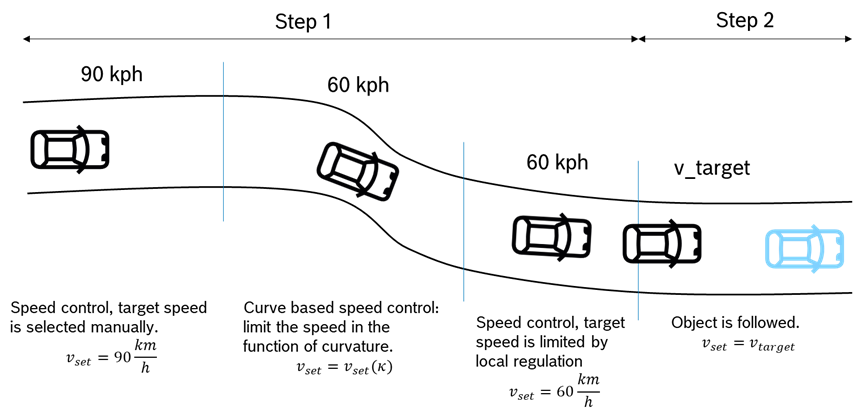
\includegraphics[width=0.8\textwidth]{lon_sa.png}}
    \caption{Function illustration, both step 1 and step 2 functionality.}
    \label{fig:lon_sa}
\end{figure}
\subsection{Longitudinal Emergency Function}
Functionality: vehicle or delegated sensors provide information about static / dynamic objects. The function decides proper strategy to stop the vehicle 
(and where to stop it). Then, this strategy is accomplished by applying proper braking force. Function use cases are shown in Figure \ref{fig:lon_em}.
Operation range: $0.0 \le v_x \le 150.0 kph$.
\begin{figure}[h]
    %\captionsetup{justification=raggedleft}
    \center{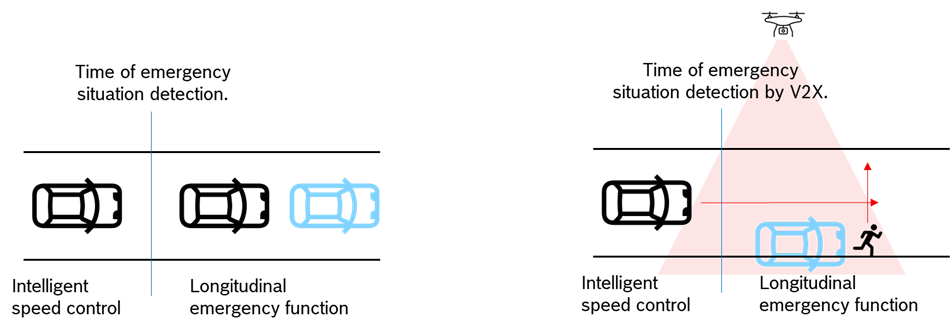
\includegraphics[width=0.8\textwidth]{lon_em.png}}
    \caption{Longitudinal emergency use cases from vehicle sensors and infrastructure sensors.}
    \label{fig:lon_em}
\end{figure}

\subsection{Lane Follow}
\begin{itemize}
    \item Step 1 functionality: vehicle is running in a lane, which is bounded by lane edges (markers or only the edge of the drivable surface) and the vehicle follows the centerline of the lane (or externally defined local trajectory). Operation range: $a_{y,max}=5 m/s^2$ , $0.0 kph \le v_x \le 150.0 kph$, $\sigma_{e_y}^2 \le 0.1 m$.
	\item Step 2 functionality: Drivable corridor is shifted due to e.g., temporarily shifted road works, which is bounded by 3D obstacles like cones, walls...etc. Vehicle (with lower dynamics) can still navigate through this drivable corridors. Operation range: $a_{y,max}=3 m/s^2$ , $0.0 kph \le v_x \le 110.0 kph$, $\sigma_{e_y)}^2 \le 0.1 m$.
\end{itemize}
\begin{figure}[h]
    %\captionsetup{justification=raggedleft}
    \center{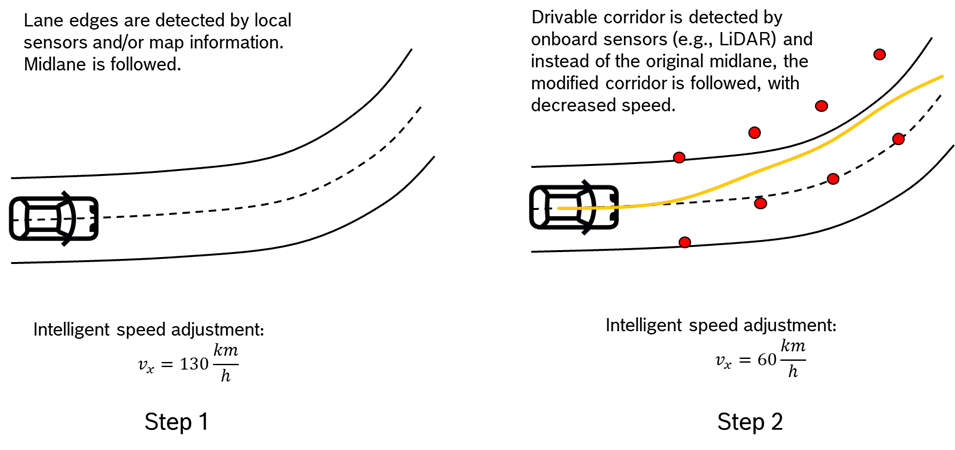
\includegraphics[width=0.8\textwidth]{lat_comf.png}}
    \caption{Lane follow functionality steps and covered operation.}
    \label{fig:lat_comf}
\end{figure}

\section{Architecture Specification} \label{arch_spec}
\subsection{Comprehensive notes}
The architecture is defined based on the E2E function specifications. There are two main concepts that must be considered at all time:
\begin{itemize}
    \item fulfill E2E function requirements with the least architecture components,
    \item re-use Autoware components where possible, but keeping its number (or number/function) as low as possible.
\end{itemize}
Therefore, the work model shown in Figure \ref{fig:cycle} is strongly recommended.
\begin{figure}[h]
    %\captionsetup{justification=raggedleft}
    \center{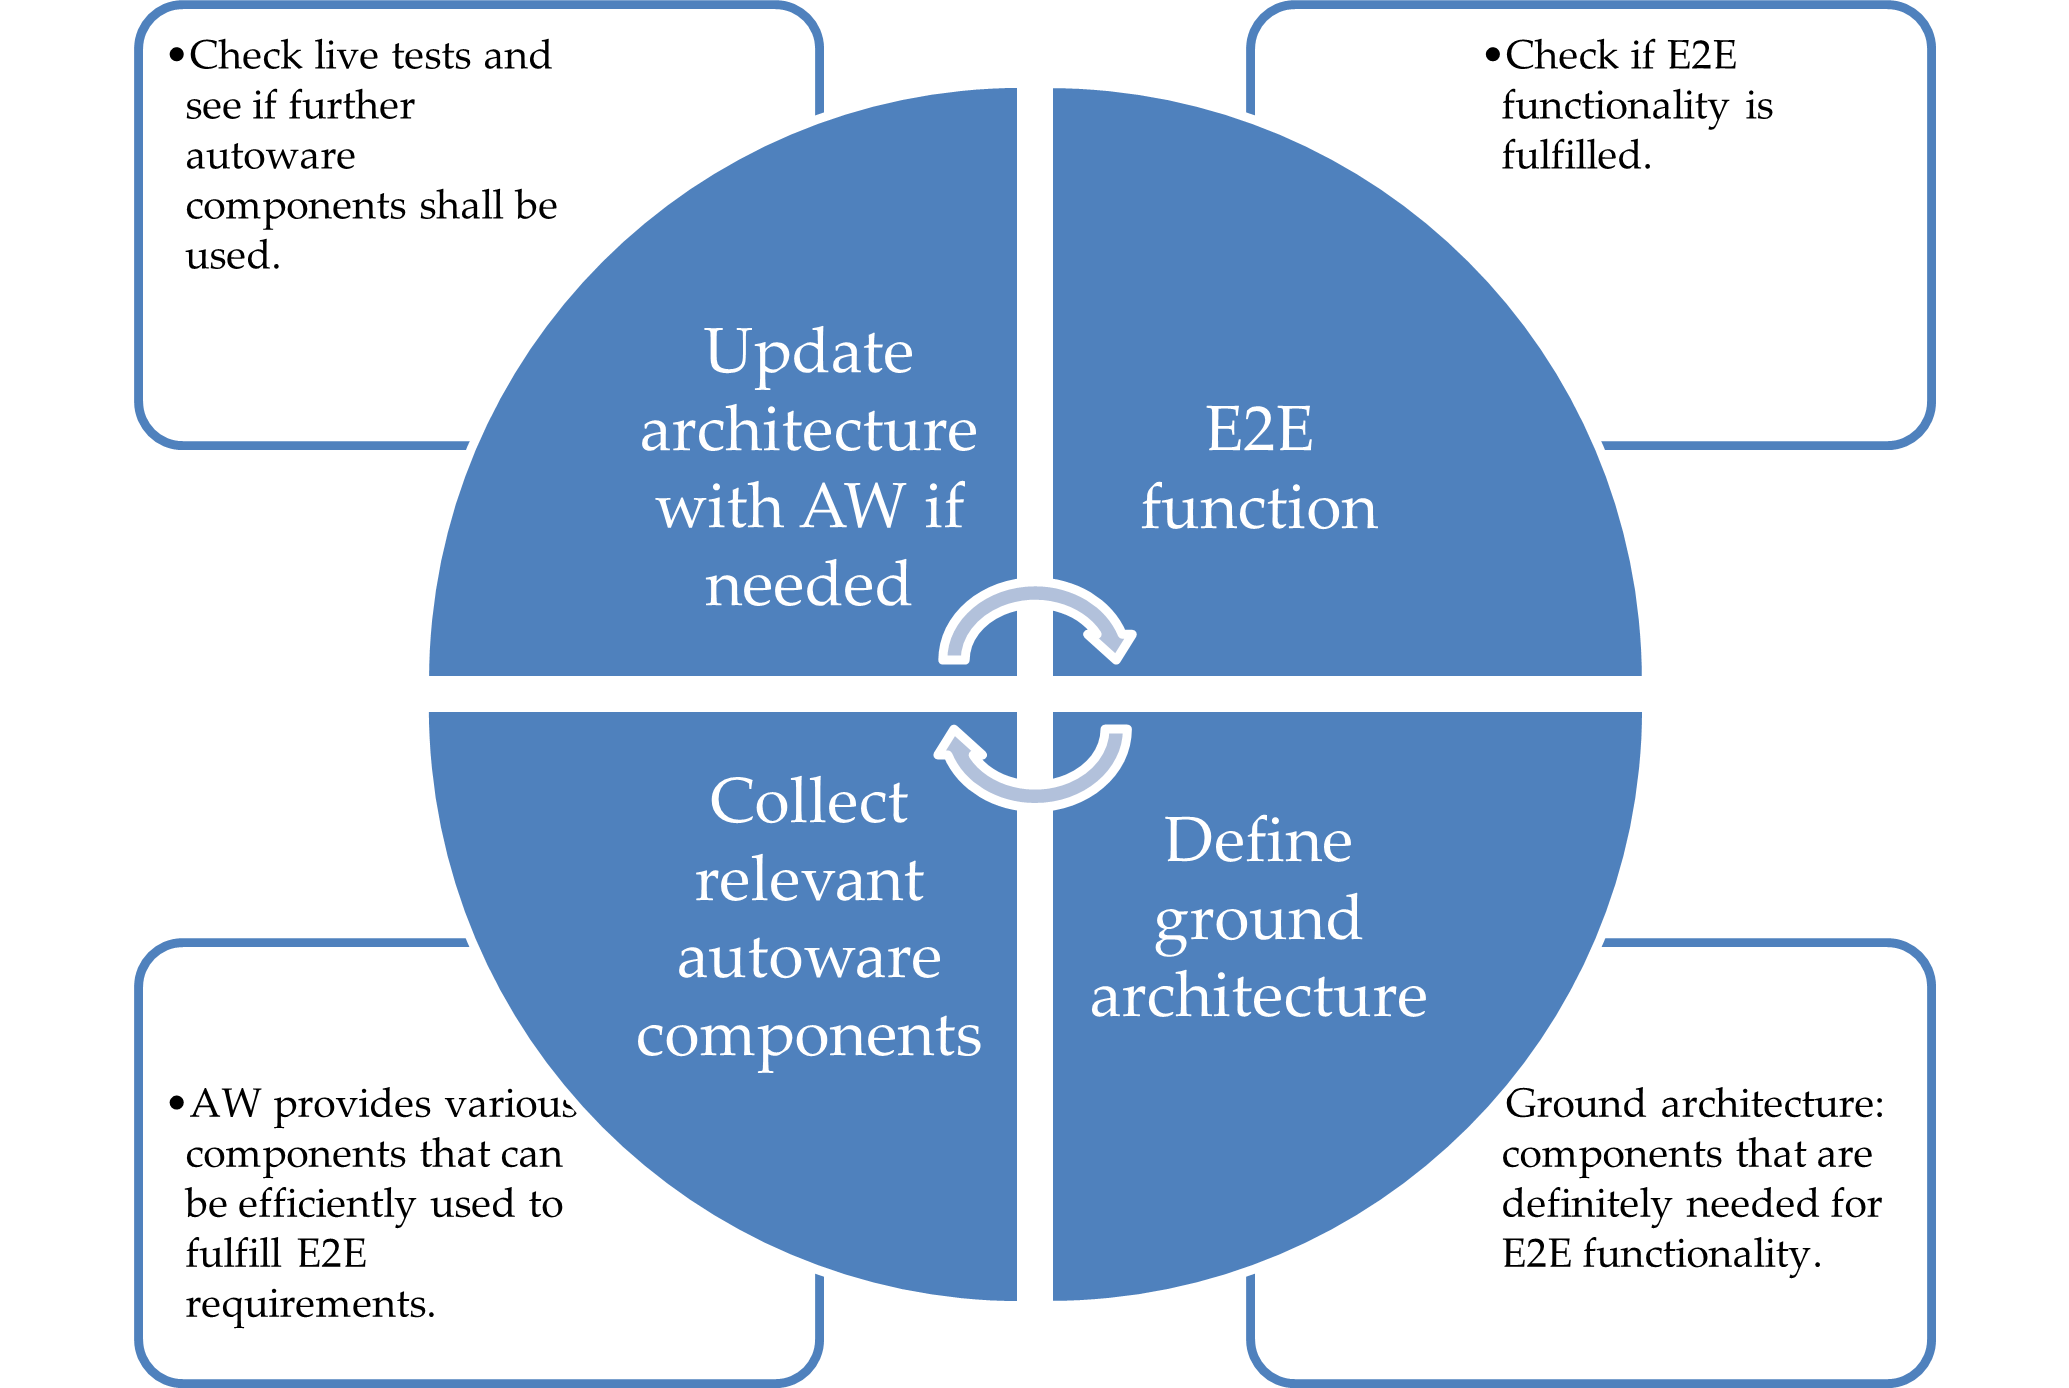
\includegraphics[width=0.8\textwidth]{cycle.png}}
    \caption{Working cycle - proposal}
    \label{fig:cycle}
\end{figure}
This concept may hinder the efficient/reliable planning of tasks regarding architecture definition, but ensures that the above two concepts are respected.

\subsection{General Architecture}
\subsubsection{High-level Black-box architecture}
\begin{figure}[h]
    %\captionsetup{justification=raggedleft}
    \center{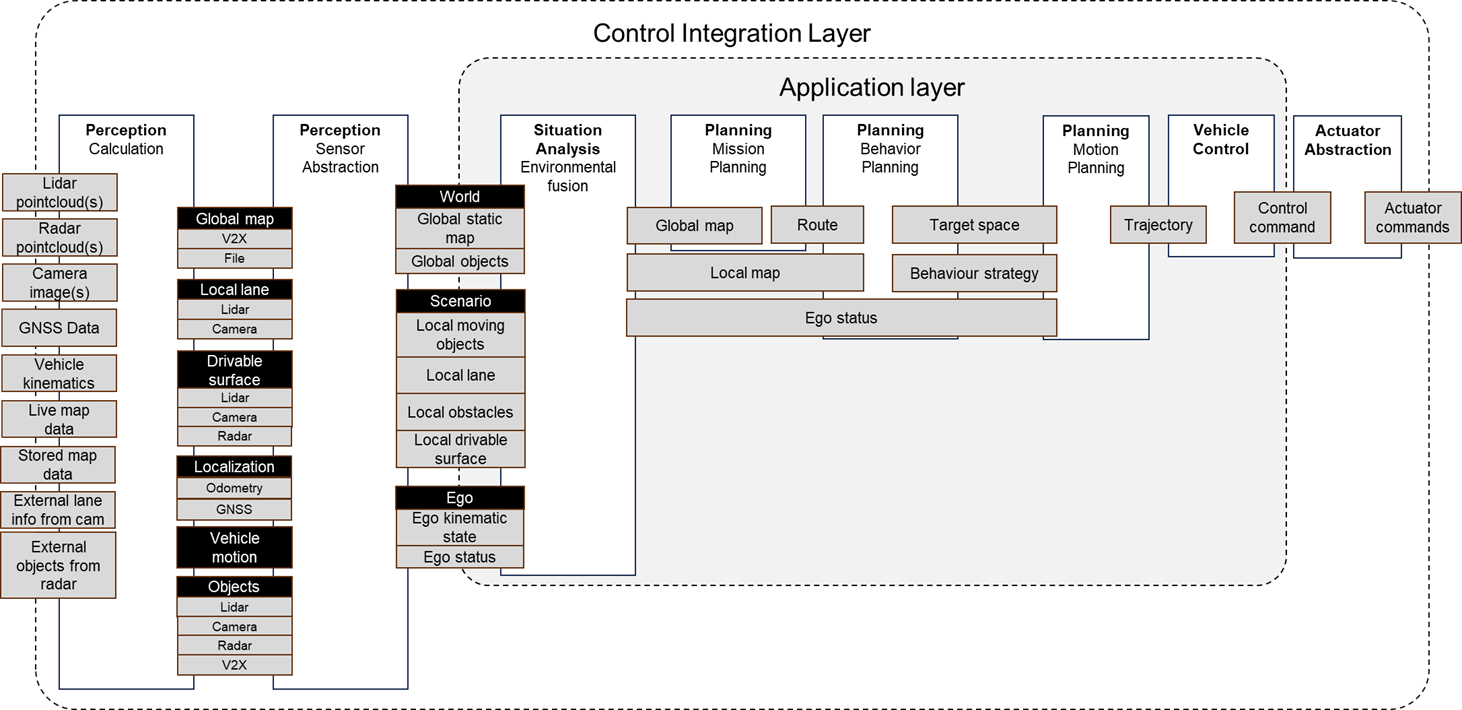
\includegraphics[width=1.0\textwidth]{gen_arch.png}}
    \caption{Black box architecture}
    \label{fig:gen_arch}
\end{figure}
\subsubsection{Gray-box architecture}
\begin{figure}[h]
    %\captionsetup{justification=raggedleft}
    \center{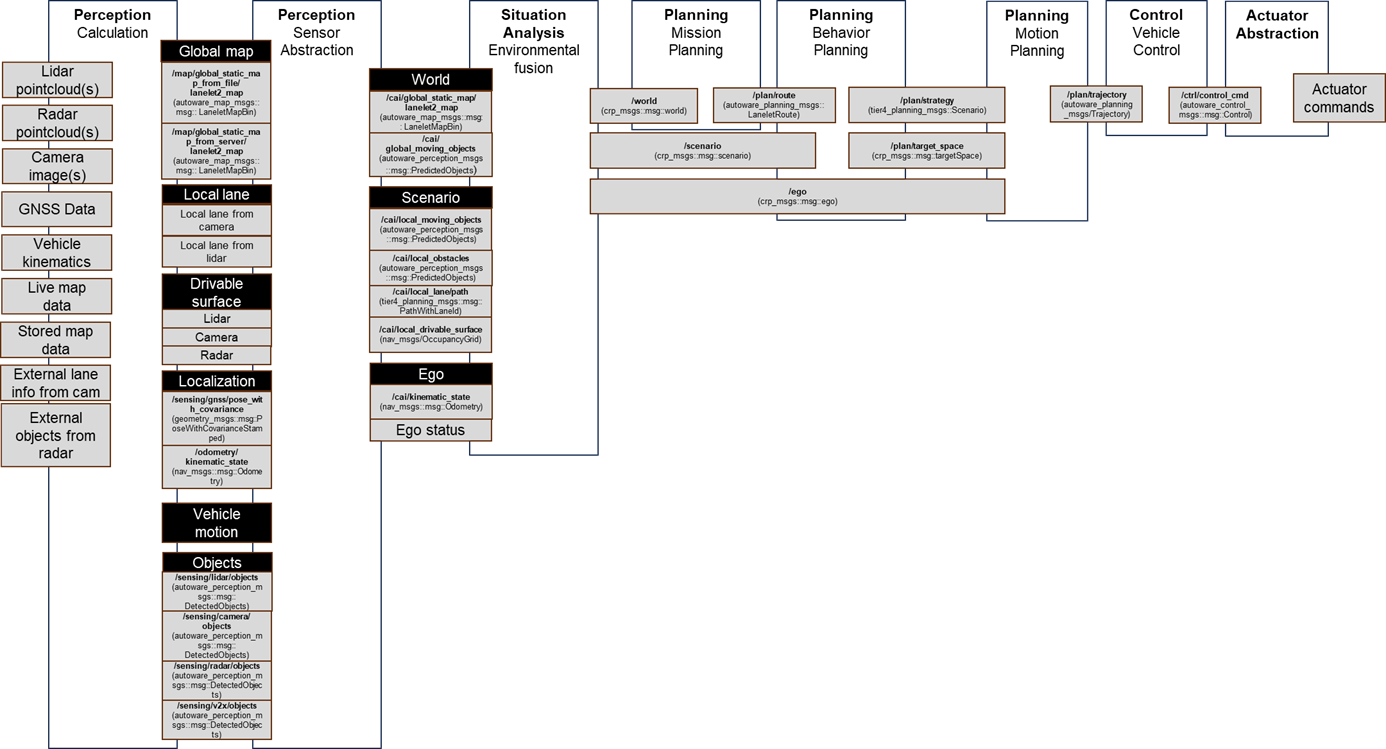
\includegraphics[width=1.0\textwidth]{gray_arch.png}}
    \caption{Gray box architecture.}
    \label{fig:gray_arch}
\end{figure}
\subsubsection{Functional (ROS2) architecture}
\begin{figure}[h]
    %\captionsetup{justification=raggedleft}
    \center{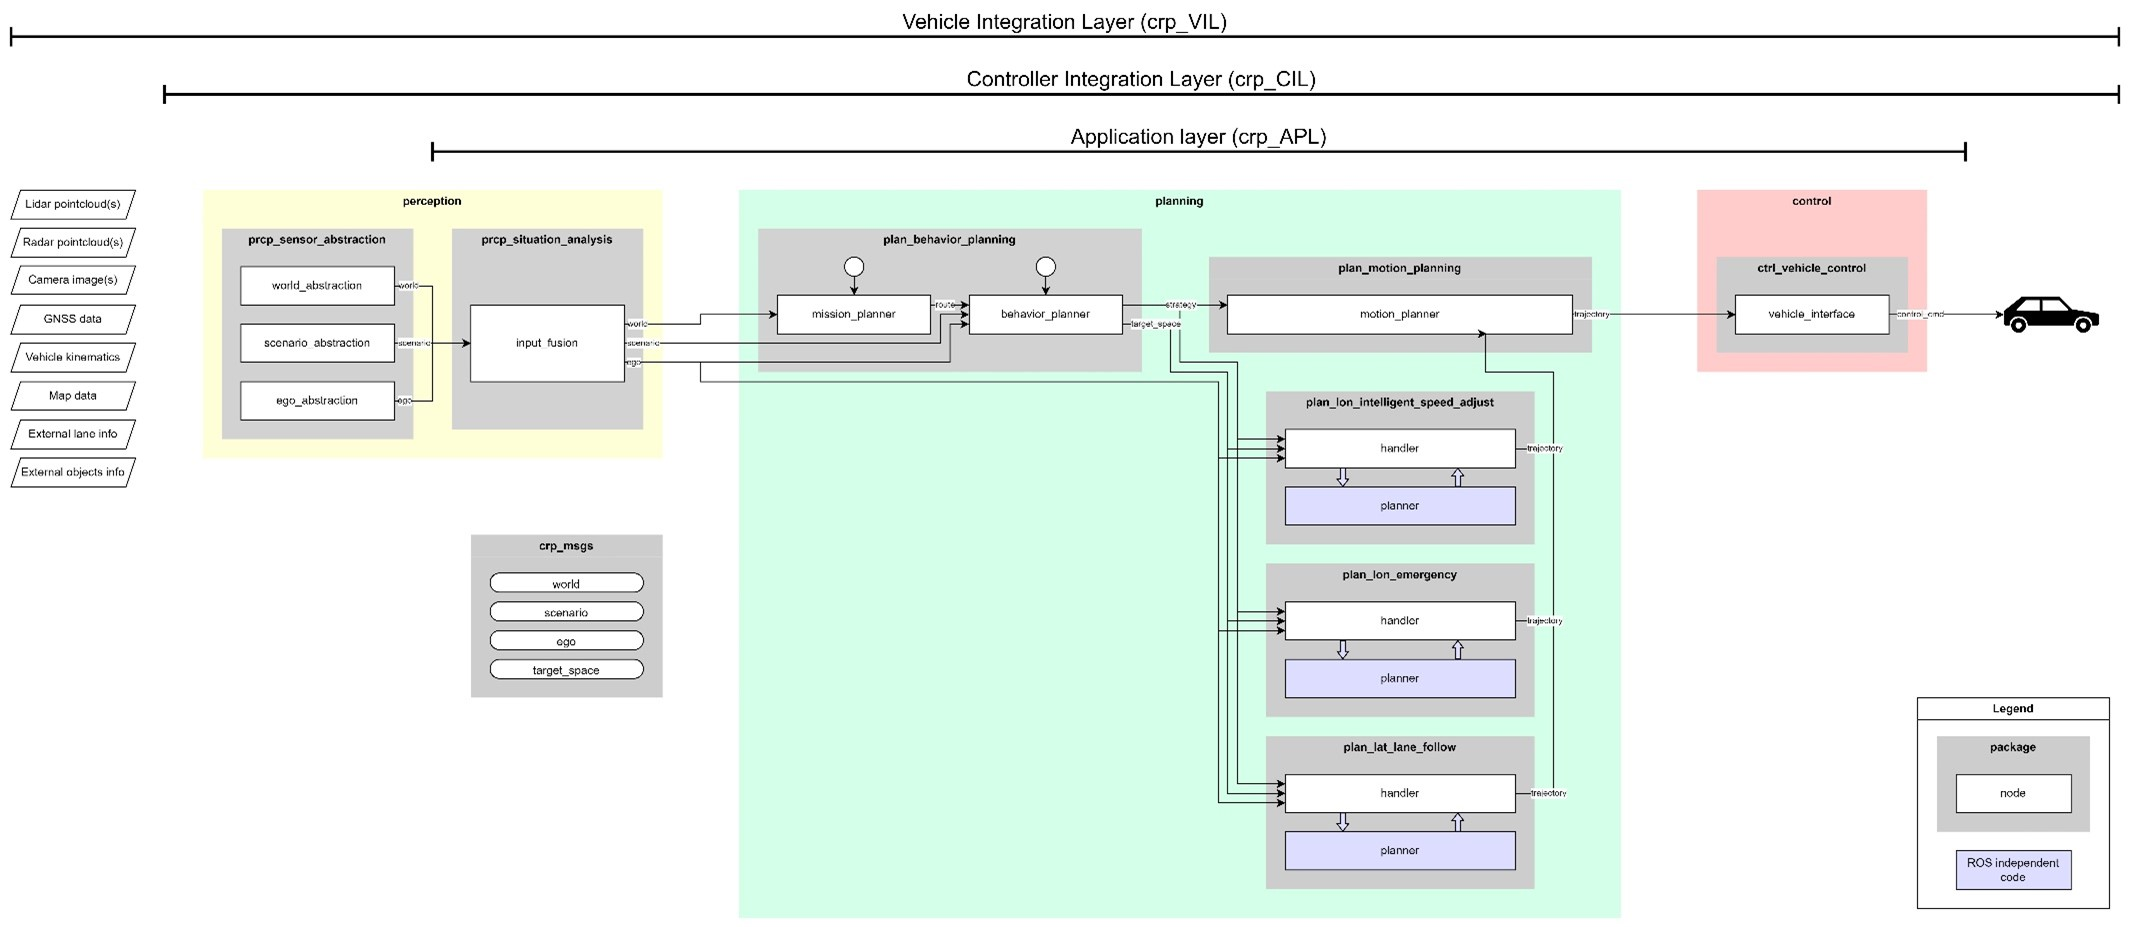
\includegraphics[width=1.0\textwidth]{func_arch.jpg}}
    \caption{Functional architecture}
    \label{fig:fun_arch}
\end{figure}

\subsection{Function Architecture Specification}
\subsubsection{Intelligent Speed Adjustment}
Step 1 architecture is shown in Figure \ref{fig:sa_step1}.
\begin{figure}[h]
    %\captionsetup{justification=raggedleft}
    \center{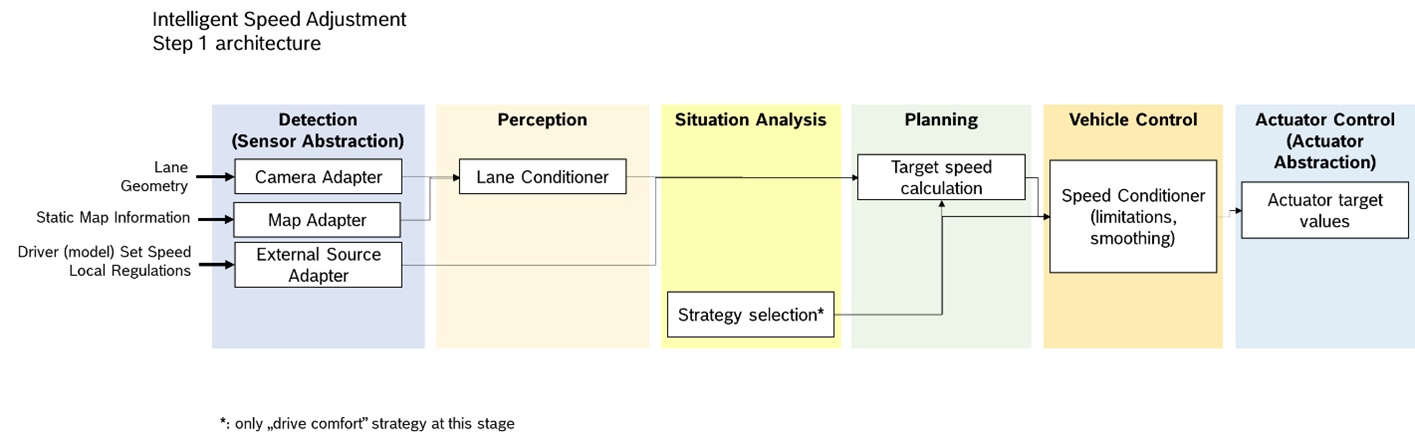
\includegraphics[width=0.8\textwidth]{gen_arch_sa_step1.png}}
    \caption{Architecture components of step 1 functionality of ISA}
    \label{fig:sa_step1}
\end{figure}
Note: even if we only control the vehicle longitudinally, the lateral path shall be filled with dummy values. Idea: add a straight line with no offset. Later, it must be solved that the vehicle is longitudinally controlled by the system, but laterally by the driver.
\newline Step 2 architecture is shown in Figure \ref{fig:sa_step2}.
\begin{figure}[h]
    %\captionsetup{justification=raggedleft}
    \center{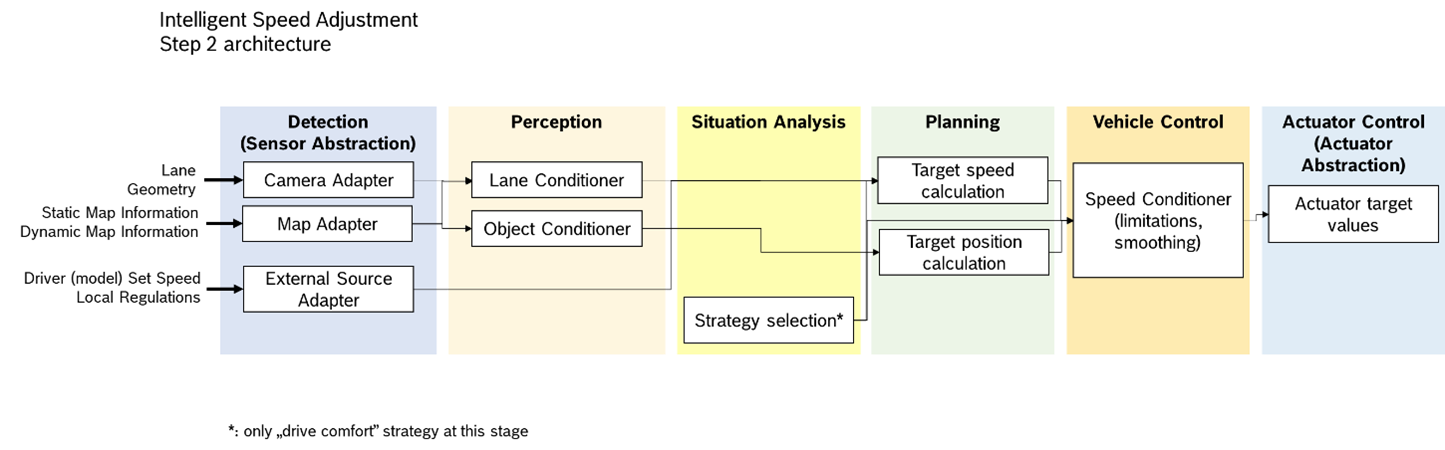
\includegraphics[width=0.8\textwidth]{gen_arch_sa_step2.png}}
    \caption{Architecture components of step 2 functionality of ISA}
    \label{fig:sa_step2}
\end{figure}

\subsubsection{Longitudinal emergency function}
Based on distributed sensor data calculate the trigger of the emergency scenario. Corresponding architecture is shown in Figure \ref{fig:em_step1}.
\begin{figure}[h]
    %\captionsetup{justification=raggedleft}
    \center{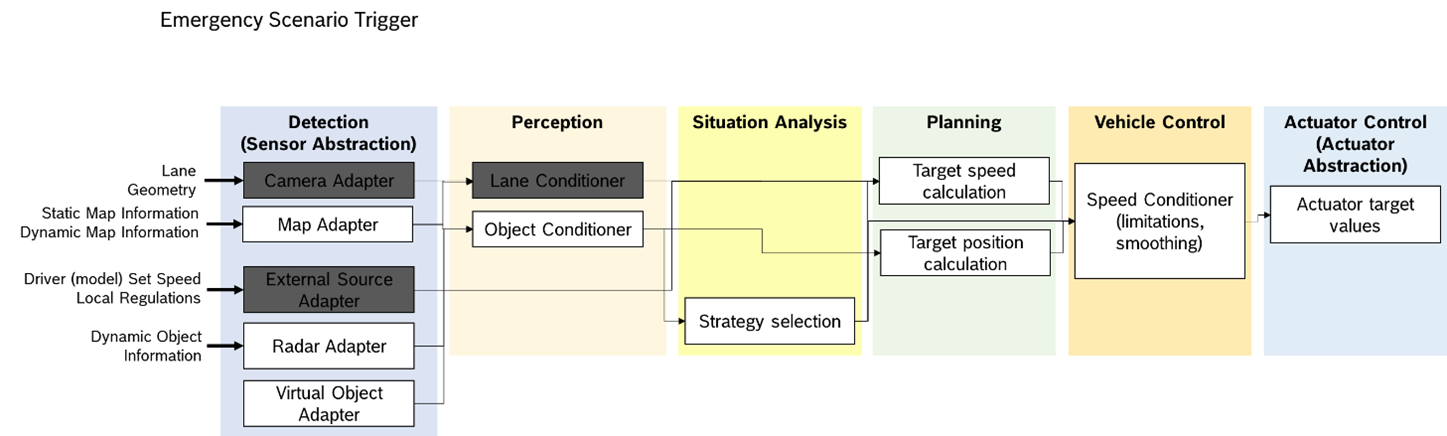
\includegraphics[width=0.8\textwidth]{gen_arch_em.png}}
    \caption{Architecture components of step 1 longitudinal emergency function.}
    \label{fig:em_step1}
\end{figure}

\subsubsection{Lane Follow}
Lane follow functional architecture is shown in Figure \ref{fig:lat_step1}.
\begin{figure}[h]
    %\captionsetup{justification=raggedleft}
    \center{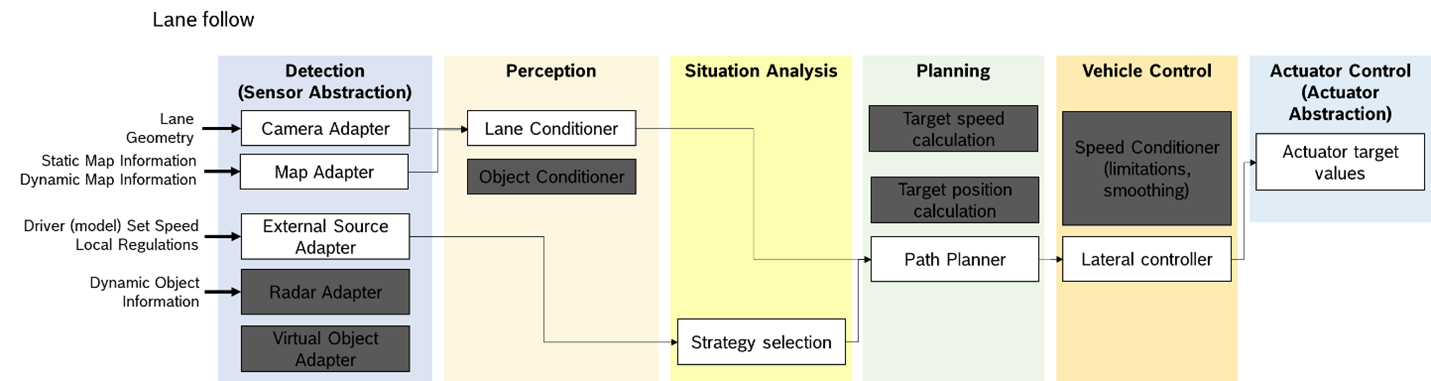
\includegraphics[width=0.8\textwidth]{gen_arch_lat_step1.png}}
    \caption{Architecture components of step 1 functionality of LF (lane follower) without behaviour layer.}
    \label{fig:lat_step1}
\end{figure}
Lane follow architecture consists of new components of path planner, that takes geometry information of the road, and plans a smooth (drivable) path, 
which is then handed over to the lateral controller component. This controller controls only the lateral movement of the vehicle, producing output to the 
actuator control (i.e., steering angle).
Note: route input comes from mission planner, which is currently not part of the architecture. During integration process, it may be extended.
Step 2 architecture is shown in Figure \ref{fig:lat_step2}.
\begin{figure}[h]
    %\captionsetup{justification=raggedleft}
    \center{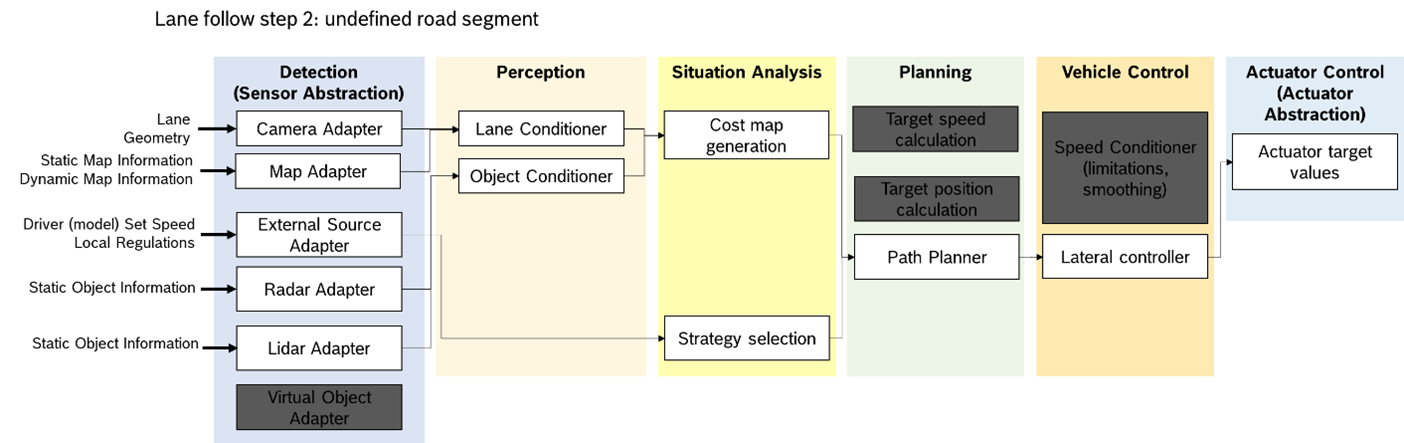
\includegraphics[width=0.8\textwidth]{gen_arch_lat_step2.png}}
    \caption{Architecture components of step 2 functionality of LF (lane follower) without behaviour layer.}
    \label{fig:lat_step2}
\end{figure}

\section{Message Definitions} \label{message_definitions}
\subsection{CRP messages}
\subsubsection{crp\_msgs/msg/scenario}
This interface holds information of four main types:
\begin{itemize}
    \item local moving objects: highest layer which is associated with other objects that move around the ego vehicle, such as other vehicles, pedestrians, animals...etc.
    \item local obstacles: static items that are located around the ego vehicle. 
    \item local lanes: the lanes that are mainly marked by painted markers and form the static driving corridors. 
    \item local drivable surface: the most indefinite representation of the local environment, in the form of a generic occupancy grid.
\end{itemize}
This interface type (in contrast to globally defined 'world' interface) must contain data with as high accuracy as possible.
Message definition:
\begin{lstlisting}
    std_msgs/Header header

    autoware_perception_msgs/PredictedObject[] local_moving_objects
    autoware_perception_msgs/PredictedObject[] local_obstacles
    tier4_planning_msgs/PathWithLaneId[] lanes
    // traffic rules information to be added
    nav_msgs/OccupancyGrid free_space
    std_msgs/Float32 maximum_speed
\end{lstlisting}
Note: the traffic rules collect all types of information that are coming from the static rules and can impact the selected bahviour. These are like:
\begin{itemize}
    \item stop lines (stop signs and lines)
    \item speed limitation
    \item traffic light information (semi-static)...etc.
\end{itemize}
\begin{figure}[h]
    %\captionsetup{justification=raggedleft}
    \center{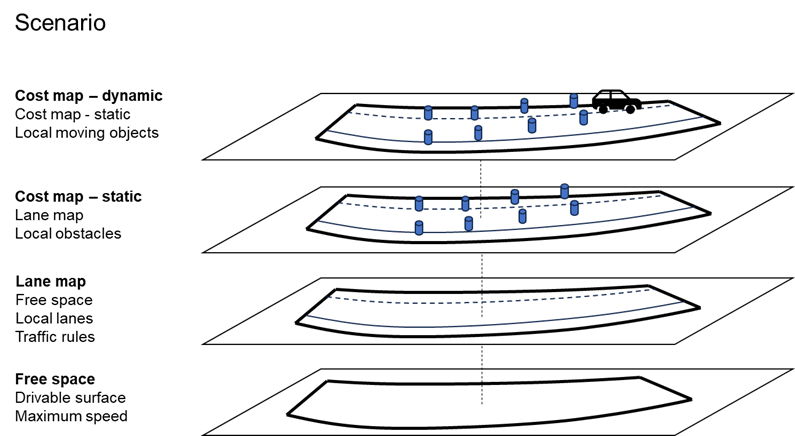
\includegraphics[width=0.8\textwidth]{scenario.png}}
    \caption{Illustration of the scenario layers.}
    \label{fig:scenario}
\end{figure}

\subsubsection{crp\_msgs/msg/world}

\subsubsection{crp\_msgs/msg/ego}
This interface contains every relevant information about the ego vehicle:
\begin{itemize}
    \item pose: position, orientations and uncertainty
    \item velocity: linear and angular
    \item acceleration: linear and angular
    \item wheel angle
\end{itemize}
Message definition:
\begin{lstlisting}
    std_msgs/Header header

    geometry_msgs/PoseWithCovariance pose
    geometry_msgs/TwistWithCovariance twist
    geometry_msgs/AccelWithCovariance accel
    float32 wheel_angle
\end{lstlisting}

\subsection{Tier4 messages in use}
\subsubsection{Path}
This is a tier4 autoware message extension, with the following definition:
\begin{lstlisting}
    std_msgs/Header header

    tier4_planning_msgs/PathPoint[] points
    nav_msgs/OccupancyGrid drivable_area
\end{lstlisting}

\subsubsection{Path point}
\begin{lstlisting}
    uint8 REFERENCE=0
    uint8 FIXED=1
    geometry_msgs/Pose pose
    geometry_msgs/Twist twist
    uint8 type
\end{lstlisting}

\subsubsection{Trajectory}
\begin{lstlisting}
    std_msgs/Header header
    tier4_planning_msgs/TrajectoryPoint[] points
\end{lstlisting}

\subsubsection{Trajectory point}
\begin{lstlisting}
    geometry_msgs/Pose pose
    geometry_msgs/Twist twist
    geometry_msgs/Accel accel
\end{lstlisting}

\section{Using the Platform} \label{using_platform}
\subsection{Installation (source)}
Create workspace and clone the repository:
\begin{lstlisting}
    mkdir -p crp_ws/src
    cd crp_ws/src
    git clone https://github.com/jkk-research/CooperativeResearchPlatform.git --recurse-submodules
\end{lstlisting}
Install dependencies and build the workspace:
\begin{lstlisting}
    cd ..
    rosdep install --from-paths src --ignore-src -y
    colcon build --symlink-install
\end{lstlisting}

\subsection{Using it in a docker container}
\subsubsection{Docker container}
The platform can be used in a docker container. The docker is available here: https://hub.docker.com/repository/docker/anonymdavid/crp/general
\subsubsection{Building the docker}
Alternatively the autoware docker can be built using the script inside the autoware repository. The docker container is built on top of the autoware docker (ghcr.io/autowarefoundation/autoware:latest-devel-cuda). Autoware and CRP should be built for the same platform type (amd64/arm64).
\newline
The container can be build to ARM64 platform:
\begin{lstlisting}
    cd CooperativeResearchPlatform
    ./docker/build_arm64.sh
\end{lstlisting}
\subsubsection{Running the docker}
The docker can be run with the following command:
\begin{lstlisting}
    docker run -it --rm --network host --ipc host --pid host --device /dev/leaf0 --device /dev/leaf1 crp_arm64:latest
\end{lstlisting}
This way the docker shares the network with the host and has access to the kvaser CAN device.

\section{Coding rules} \label{sec:coding_rules}
\subsection{Naming convention}
\begin{itemize}
    \item Use camel case everywhere if not stated otherwise - example: \emph{latLaneFollow}
    \item Classes and structs should start with upper case letter - example: \emph{MotionHandler}
    \item Methods should be camel case (starting with small case) - example: \emph{scenarioCallback}
    \item Method arguments have no prefix/suffix, they must be given with camel case - example: \emph{plannerInput}
    \item Constant variables should be all capital letters. Instead of camel case the words should be separated with '\_' - example: \emph{MAX\_SPEED}
    \item In classes all member variables should start with the 'm\_' prefix - example: \emph{m\_vxEgo}
    \item The runtime calibratable parameters should start with the 'p\_' prefix - example: \emph{p\_mainThreshold}
    \item In special cases (e.g., subscribers/publishers) extra name tags can be added with lower case, separated by underscore - example: \emph{m\_sub\_strategy\_}
    \item Pointers should comply with the previous rules but should have a '\_' suffix - example: \emph{m\_sub\_strategy\_}
    \item Namespaces should be fully lower case - example: \emph{crp}
    \item Maximum namespace depth should be 3
    \item File and folder names should be camel case where it is not restricted (e.g. ROS2 naming rules)
\end{itemize}

\subsection{Cplusplus}
\subsubsection{General}
\begin{itemize}
    \item Header and source files should be separated ('include' folder for headers and 'src' folder for source files)
    \item Header files should only contain declarations, the definitions should be in a source file that includes the header
    \item If applicable, include further header files in the main header file, not in the source file (source file (i.e., cpp) should only include its own declaration header)
    \item Functional code should be included in a separate cmake file (with .cmake extension), which is then included in the main CMakeList.txt (this way, cmake file with functional sources is ROS agnostic)
\end{itemize}

\subsubsection{Header files}
Every header file should…
\begin{itemize}
    \item have the '.hpp' extension,
    \item have header guards (\#ifndef, \#define, \#endif) and it should be all capitals,
    \item contain max. one class.
\end{itemize}

\subsubsection{Source files}
Every source file should…
\begin{itemize}
    \item have the “.cpp” extension.
\end{itemize}

\subsection{ROS2}
\subsubsection{Packages}
Non-driver package names should start with and abbreviation of the following categories:
\begin{itemize}
    \item prcp (perception)
    \item plan (planning)
    \item ctrl (control)
\end{itemize}
All dependencies must be set in the package.xml and in the CMakeList.txt.
\newpage

\section{Package documentations}
\subsection{pacmod\_extender}
\subsubsection{Purpose}
The purpose of this package is to extend the default pacmod capabilities on the Lexus vehicle by decoding CAN messages or calculating new data from the inputs. The package is designed to work seamlessly with the already existing pacmod3 system.
\subsubsection{Usage}
The package can be used by running the executable node. This way it uses the default namespace for subscriptions and publishers:
\begin{lstlisting}
    ros2 run pacmod_extender pacmod_extender_node
\end{lstlisting}
The other way is to use the launcher. This launcher is tailored for the Lexus vehicle by giving the executable the necessary namespace to match the other components:
\begin{lstlisting}
    ros2 launch pacmod_extender pacmod_extender.launch.py
\end{lstlisting}

\subsubsection{IO}
Input topics are given in Table \ref{tab:pacmod_input}, outputs are given in Table \ref{tab:pacmod_output}.
\begin{table}[!h]
    \captionsetup{justification=centering}
    \normalsize
        \caption{\label{tab:pacmod_input} Pacmod extender inputs.}
        \begin{tabular}{ | c | c | c |}
            \hline
            \textbf{Data} & \textbf{Message name} & \textbf{Message Type} \\
            \hline
            Raw can data & pacmod\slash can\_tx & can\_msgs\slash msg \slash Frame \\
            \hline
            Vehicle test & vehicle\_status & geometry\_msgs\slash msg\slash TwistStamped \\
            \hline
        \end{tabular}
\end{table}
\begin{table}[!h]
    \captionsetup{justification=centering}
    \normalsize
        \caption{\label{tab:pacmod_output} Pacmod extender output.}
        \begin{tabular}{ | c || c | c |}
            \hline
            \textbf{Data} & \textbf{Message name} & \textbf{Message Type} \\
            \hline
            Linear acceleration & pacmod/linear\_accel\_rpt & pacmod3\_msgs/msg/LinearAccelRpt \\
            \hline
            Calculated yaw rate & pacmod/yaw\_rate\_calc\_rpt & Pacmod3\_msgs/msg/YawRateRpt \\
            \hline
        \end{tabular}
\end{table}
\subsubsection{Inner workings}
The main functionality is the decoding of previously not used CAN messages. The decodings are defined in the PacmodDefinitions class. Every message has a decode method that requires the CAN message as parameter. The message IDs are stored as constants in the class.
The PacmodExtender class is the main class that is executed as a node. It subscribes to the inputs, uses the PacmodDefinitions class to decode the CAN messages and outputs the new messages. The output rate of every message depends on the input frequencies. Every output value is in SI units.
Decodings:
\begin{itemize}
	\item Linear acceleration
	\item longitudinal, lateral, vertical acceleration in m/s
\end{itemize}
Calculations:
\begin{itemize}
	\item Yaw rate $\psi= v_\xi  tan(\frac{\alpha_f}{L_w})$, where $\psi$ is the yaw rate, $\alpha_f$ is the front road-wheel angle and $L_w$ is the wheelbase.
\end{itemize}


\subsection{duro\_gps\_launcher}
\subsubsection{Purpose}
The purpose of this package is to launch the duro GPS driver. The driver is in a separate repository included as a subrepository. It also contains a node (duro\_topic\_converter) that converts the duro GPS topics to the predefined CRP topics.
\subsubsection{Usage}
The package only contains the launcher for the driver. This can be started as follows:
\begin{lstlisting}
    ros2 launch duro_gps_launcher duro.launch.py
\end{lstlisting}
\subsubsection{Launch parameters}
The parameters of the launcher are given in Table \ref{tab:duro_gps_launcher}. The default values are set for the Lexus vehicle.
\begin{table}[!h]
    \captionsetup{justification=centering}
    \normalsize
    \caption{\label{tab:duro_gps_launcher} Duro gps launcher parameters.}
    \begin{tabular}{| l | l | l |}
        \hline
        \textbf{Name} & \textbf{Default value} & \textbf{Description} \\
        \hline
        duro\_namespace  & gps/duro       & Namespace for the Novatel GPS \\
        \hline
        duro\_ip         & 192.168.10.11  & IP address of the Duro GPS \\
        \hline
        duro\_port       & 5555           & Port of the Novatel GPS \\
        \hline
    \end{tabular}
\end{table}


\subsection{novatel\_gps\_launcher}
\subsubsection{Purpose}
The purpose of this package is to launch the novatel GPS driver. The driver is in a separate repository included as a subrepository. It also contains a node (novatel\_topic\_converter) that converts the novatel GPS topics to the predefined CRP topics.
\subsubsection{Usage}
The package only contains the launcher for the driver. This can be started as follows:
\begin{lstlisting}
    ros2 launch novatel_gps_launcher novatel.launch.py
\end{lstlisting}
\subsubsection{Launch parameters}
The parameters of the launcher are given in Table \ref{tab:novatel_gps_launcher}. The default values are set for the Nissan leaf vehicle.
\begin{table}[!h]
    \captionsetup{justification=centering}
    \normalsize
    \caption{\label{tab:novatel_gps_launcher} Novatel gps launcher parameters.}
    \begin{tabular}{| l | l | l |}
        \hline
        \textbf{Name} & \textbf{Default value} & \textbf{Description} \\
        \hline
        novatel\_namespace  & gps/nova          & Namespace for the Novatel GPS \\
        \hline
        novatel\_ip         & 192.168.1.11      & IP address of the Novatel GPS \\
        \hline
        novatel\_port       & 3002              & Port of the Novatel GPS \\
        \hline
        novatel\_imu\_frame & /nissan9/nova/imu & IMU frame id of the Novatel GPS \\
        \hline
        novatel\_frame\_id  & /nissan9/nova/gps & Frame id of the Novatel GPS \\
        \hline
    \end{tabular}
\end{table}


\subsection{lanelet\_handler}
\subsubsection{Purpose}
The purpose of this package is to load and publish a lanelet2 map to a specified topic using the autoware lanelet2 library.
\subsubsection{Usage}
The package can be used by the provided launcher:
\begin{lstlisting}
    ros2 launch lanelet_handler laneletFileLoader.launch.py
\end{lstlisting}
\subsubsection{Launch parameters}
Launch parameters are given in Table \ref{tab:lanelet_handler}.
\begin{table}[!h]
    \centering
    \captionsetup{justification=centering}
    \normalsize
    \caption{\label{tab:lanelet_handler} Launch parameters.}
    \begin{tabular}{| l | l | l |}
        \hline
        \textbf{Name} & \textbf{Default value} & \textbf{Description} \\
        \hline
        map\_file\_path           &                                       & Path to the lanelet2 map file \\
        \hline
        map\_output\_topic        & /map/global\_static\_map\_from\_file/ & Output topic for the map binary \\
                                  & lanelet2\_map                         &  \\
        \hline
        map\_frame\_id            & map                                   & Frame id of the lanelet2 map \\
        \hline
        map\_visualization\_topic & /map/global\_static\_map\_from\_file/ & Frame id of the lanelet2 map \\
                                  & lanelet2\_map\_visualization          &  \\
        \hline
    \end{tabular}
\end{table}


\subsection{mcap\_rec}
\subsubsection{Purpose}
This package contains scipts for recording all the necessary topics of the project.
\subsubsection{Usage}
The package can be used by the provided launchers:
\begin{lstlisting}
    ros2 launch mcap_rec recordLexus.launch.py tag:=name_of_the_recording
\end{lstlisting}
\subsubsection{Recorded params}
Each launcher has a different preset for which topics to record. The recorded topics are defined in the etc folder in txt files.


\subsection{nissan\_can\_driver}
\subsubsection{Purpose}
The purpose of this package is to publish the vehicle status (speed, steering) to topics and receive control commands from topics to control the vehicle.
\subsubsection{Usage}
The package can be used by the provided launcher:
\begin{lstlisting}
    ros2 launch nissan_can_driver can_driver_kvaser.launch.py
\end{lstlisting}
In the current implementation a kvaser device with 2 channels is used for the communication. On the first channel the CAN data is received from the vehicle and on the second channel the control commands are sent to the controllers.
\subsubsection{Launch parameters}
Launch parameters are given in Table \ref{tab:nissan_can_driver_params}.
\begin{table}[!h]
    \centering
    \captionsetup{justification=centering}
    \normalsize
    \caption{\label{tab:nissan_can_driver_params} Launch parameters.}
    \begin{tabular}{| l | l | l |}
        \hline
        \textbf{Name} & \textbf{Default value} & \textbf{Description} \\
        \hline
        autoware\_control\_input & True  & Whether to use autoware or standard type \\
                                 &       & input message for control \\
        \hline
        kvaser\_hardware\_id     & 11162 & HW ID of the kvaser device used for CAN communication \\
        \hline
    \end{tabular}
\end{table}
\subsubsection{IO}
Input topics are given in Table \ref{tab:nissan_can_driver_inputs}.
\begin{table}[!h]
    \centering
    \captionsetup{justification=centering}
    \normalsize
    \caption{\label{tab:nissan_can_driver_inputs} Launch parameters.}
    \begin{tabular}{| l | l | l |}
        \hline
        \textbf{Name} & \textbf{Message type} & \textbf{Description} \\
        \hline
        /ctrl/control\_cmd  & autoware\_control\_msgs/msg/Control & Control input topic if \textit{autoware\_control\_input}  \\
                            &                                     & is set to true                                            \\
                            &                                     & Contains speed and steering commands                      \\
        \hline
        /ctrl/speed\_cmd    & std\_msgs/msg/Float32                & Control input topic if \textit{autoware\_control\_input} \\
                            &                                     & is set to true                                            \\
                            &                                     & Contains speed command (m/s)                              \\
        \hline
        /ctrl/steering\_cmd & std\_msgs/msg/Float32                & Control input topic if \textit{autoware\_control\_input} \\
                            &                                     & is set to true                                            \\
                            &                                     & Contains steering command (tire angle, rad)               \\
        \hline
    \end{tabular}
\end{table}

\bibliography{refs}% common bib file
%% if required, the content of .bbl file can be included here once bbl is generated
%%\input sn-article.bbl


\end{document}
